\documentclass[doctor]{USTBThesis}

\begin{document}

%论文信息
% !Mode:: "TeX:UTF-8"

%ѧУ����
\university{�����Ƽ���ѧ}{University of Science and Technology Beijing}

%ѧԺ
\school{��ľ�뻷������ѧԺ}{School of Civil and Environmental Engineering}

%רҵ
\major{������ѧ}{Fluid Dynamics}

%������Ŀ��ǰ��������������Ӣ�ģ��������Ǹ�������Ӣ��
\thesistitle{�����Ƽ���ѧ��ʿѧλ����ģ���д���о�}{Research of USTB Doctor Thesis \LaTeX Model Writing}{\LaTeX ��ѧϰӦ��}{Use and Study of \LaTeX}

%����
\thesisauthor{С�һ�}{JeffHugh}

%ѧ��
\authorid{B20160001}

% ָ����ʦ��������Ϊָ����ʦ��λ
\teacher{����ʦ}{Teacher 1}{�����Ƽ���ѧ}{����}

% ��ָ����ʦ��������Ϊ��ָ����ʦ��λ
\subteacher{����ʦ}{Teacher 2}{�����Ƽ���ѧ}{������}

% �����
\category{TP312}

%�����ύ����
\thesisdate{2016}{04}{25}


%论文封面
% !Mode:: "TeX:UTF-8"

%���ķ���
\newcommand{\makecover}{%
    ~
    \vspace{5em}

    \begin{tabular}[H]{p{60pt} p{1em}}
    & \linespread{0.8}\selectfont \zihao{-2} \ThesisTitleCN \\	%��Ӣ�Ļ���ָ�ʽ����
    &\\
    &\linespread{0.8}\selectfont \zihao{-2} \AuthorCN \\
    &\\
    &\linespread{0.8}\selectfont \zihao{-2} �����Ƽ���ѧ
    \end{tabular}
}
\makecover
\pagestyle{empty}

\newpage
\pagestyle{empty}

%���ĵڶ�����
\begin{titlepage}
\begin{center}

\hfill
\newlength{\Mycode}
\settowidth{\Mycode}{�� \qquad ����\qquad �� \qquad �� \qquad}
\begin{minipage}[t]{\Mycode}
�� \qquad ����\uline{\qquad �� \qquad �� \qquad}
\end{minipage}
\vspace{140mm}

%����������
\centerline{\zihao{-3} ������Ŀ��\zihao{-2} \textbf{\ThesisTitleCN}} \par    %ǿ��ֻʹ��һ��
%\zihao{-3} ������Ŀ��\zihao{-2} \textbf{\ThesisTitleCN} \par     %���Է���
\vspace{10mm}

%���ĸ����⣬û����ע�͵�
\centerline{\zihao{3} ���� \textbf{\ThesisSubTitleCN}} \par
\vspace{30mm}

\zihao{-3}

\begin{tabular}{rc}
ѧ \qquad �ţ�& \underline{\makebox[5cm]{\StudentID}} \\
�� \qquad �ߣ�& \underline{\makebox[5cm]{\AuthorCN}}\\
רҵ���ƣ�& \underline{\makebox[5cm]{\MajorCN}}
\end{tabular}
\vspace{10mm}

\ThesisYear �� \ThesisMonth �� \ThesisDay ��

\end{center}
\end{titlepage}

\newpage
\pagestyle{empty}

%���ĵ�������
\begin{titlepage}
\begin{center}
\qquad
\vspace{10mm}

\zihao{-2}
%��������������
\centerline{\ThesisTitleCN} \par    %ǿ��ֻʹ��һ��
%\ThesisTitleCN \par     %���Է���
\vspace{10mm}

%�������ĸ����⣬û����ע�͵�
\centerline{\ThesisSubTitleCN} \par
\vspace{20mm}

%����Ӣ��������
\centerline{\ThesisTitleEN} \par    %ǿ��ֻʹ��һ��
%\ThesisTitleEN \par     %���Է���
\vspace{10mm}

%����Ӣ�ĸ����⣬û����ע�͵�
\centerline{\ThesisSubTitleEN} \par
\vspace{40mm}

\zihao{-4}
���������\AuthorCN \par
\vspace{3mm}
ָ������������\TeacherCN \par
\vspace{3mm}
\UniversityCN \SchoolCN \par
\vspace{3mm}
���� 100083���й� \par
\vspace{8mm}

Doctor Degree Candidate��\AuthorEN \par
\vspace{3mm}
Supervisor��\TeacherEN \par
\vspace{3mm}
\SchoolEN \par
\vspace{3mm}
\UniversityEN \par
\vspace{3mm}
30 Xueyuan Road, Haidian District \par
\vspace{3mm}
Beijing 100083, P.R.CHINA

\end{center}
\end{titlepage}

\newpage
\pagestyle{empty}

%���ĵ��ķ���
\begin{titlepage}
\begin{center}

\begin{tabular}{rccrc}
\zihao{-4} ����ţ�& \zihao{5} \underline{\makebox[2cm]{\ThesisCategory}} & \qquad \qquad &\zihao{-4} �� \qquad ���� & \zihao{5} \underline{\makebox[2cm]{����}} \\
\vspace{5mm}
\zihao{-4}U D C��& \zihao{5} \underline{\makebox[2cm]{}} & \qquad \qquad & \zihao{-4} ��λ���룺 & \zihao{5} \underline{\makebox[2cm]{10008}}
\end{tabular}
\par
\vspace{30mm}

\zihao{-2} \textbf{�����Ƽ���ѧ\degreecn ѧλ����} \par
\vspace{30mm}

\zihao{4}
%����������
\centerline{ \textbf{������Ŀ��} \ThesisTitleCN } \par    %ǿ��ֻʹ��һ��
%\textbf{������Ŀ��} \ThesisTitleCN \par     %���Է���
\vspace{5mm}
%���ĸ����⣬û����ע�͵�
\centerline{ ���� \ThesisSubTitleCN} \par
\vspace{10mm}

\centerline{ \textbf{���ߣ�} \AuthorCN } \par
\vspace{70mm}

\begin{tabular}{rcrl}
\makebox[7em][s]{\textbf{ָ\hspace{\fill}��\hspace{\fill}��\hspace{\fill}ʦ��}} & \zihao{5} \underline{\makebox[3cm]{\TeacherCN \qquad \TeacherJobtitle}} & \zihao{4} \textbf{��λ��} & \zihao{5} \underline{\makebox[3cm]{\TeacherDepartment}} \\
\zihao{4} \makebox[7em][s]{\textbf{ָ��С���Ա��}} & \zihao{5} \underline{\makebox[3cm]{\SubTeacherCN \qquad \SubTeacherJobtitle}} & \zihao{4} \textbf{��λ��} & \zihao{5} \underline{\makebox[3cm]{\SubTeacherDepartment}} \\
\zihao{4} \makebox[7em][s]{\textbf{�����ύ���ڣ�}} & \multicolumn{3}{l}{\makebox[7em][s]{\ThesisYear �� \ThesisMonth �� \ThesisDay ��}} \\
\makebox[7em][s]{\textbf{ѧλ���赥λ��}} & \multicolumn{3}{l}{\makebox[7em][s]{\textbf{��\hspace{\fill}��\hspace{\fill}��\hspace{\fill}��\hspace{\fill}��\hspace{\fill}ѧ}}}
\end{tabular}

\end{center}
\end{titlepage}



\pagenumbering{Roman}
\setcounter{page}{1}

\fancypagestyle{plain}{
  \pagestyle{fancy}
}
\fancyhead{}
\fancyhead[CO]{\zihao{5}北京科技大学\degreecn 学位论文}
\fancyhead[CE]{\zihao{5} \ThesisTitleCN}

%致谢
% !Mode:: "TeX:UTF-8"

\chapter*{\centering �� \qquad л}
\addcontentsline{toc}{chapter}{��л}
�ڴ���Ҫ��л



%摘要
% !Mode:: "TeX:UTF-8"

%中文摘要
\chapter*{ 摘 \space 要 }
\addcontentsline{toc}{chapter}{摘要}
本文基于\LaTeX 使用手册,依据北京科技大学\degreecn 学位论文Word模板,


\vskip 30bp
{

    % 在关键词冒号后添加你的关键词,使用全角逗号分割
    \textbf{ \heiti \zihao{-4} 关键词:\LaTeX ,\degreecn 论文,北京科技大学}
}


%英文摘要

\chapter*{ Abstract }
\addcontentsline{toc}{chapter}{Abstract}
Based on the \LaTeX manual and referred to USTB word model for \degreeen, I

\vskip 30bp
{
    \zihao{-4}
    % 在key words冒号后添加你的关键词,使用半角逗号加空格分割
    $\mathbf{Key}$ $\mathbf{Words}$: {\LaTeX}, $\mathbf{\degreeen \space Thesis}$, $\mathbf{USTB}$
}


%序
% !Mode:: "TeX:UTF-8"
%��
\begin{USTBPreface}
���ڱ����Ƽ���ѧ������ģ����\LaTeX ������ڿհף���˴���Ŀ�����ش�����塣
\end{USTBPreface}

%目录
\tableofcontents

%表格目录,如果不使用请注释掉
\renewcommand{\listtablename}{\centering 表格清单}
\addcontentsline{toc}{chapter}{表格清单}
\listoftables

%图像目录,如果不使用请注释掉
\renewcommand{\listfigurename}{\centering 插图清单}
\addcontentsline{toc}{chapter}{插图清单}
\listoffigures

\pagestyle{fancy}
\fancyhead{}
\fancyhead[CO]{\zihao{5}北京科技大学\degreecn 学位论文}
\fancyhead[CE]{\zihao{5} \ThesisTitleCN}

%第一章
% !Mode:: "TeX:UTF-8"

\chapter{引言}
\pagenumbering{arabic}
\setcounter{page}{1}

\section{项目原因}
北京科技大学官方只提供word版本模板,但是也已陈旧不堪。希望此项目能填补北科在\TeX 方面的空白,造福科大学子。也希望更多的贝壳可以加入进来,一起Coding,欢迎提供bug、issue和code.
\section{参考资料}
请使用CTEX宏包进行编译,具体请参考CTEX使用手册。\LaTeX 的具体使用方法可以参考《一份不太简短的\LaTeXe 介绍》\cite{oetiker2002}。 \par
本项目部分借鉴自BUAAThesis ( https://github.com/BHOSC/BUAAthesis ). \par
想要了解更多关于 \LaTeX 方面的研究工作可以查看参考文献\cite{wenyayuan2012, wangyong2012, niejun2010, majiajia2014, jihongwei2011, duanmaiying2003, chenweide2009}。
\section{注意事项}
进行编译时,tex文档编码、bib文件编码和bst编码的编译方式应该是一致的, 否则会出报错。




%第二章
% !Mode:: "TeX:UTF-8"

\chapter{\LaTeX ����ʹ��}
\section{\LaTeX ������}
\LaTeX ������ʽд��LaTeX����һ�ֻ���TEX���Ű�ϵͳ������������ѧ����˹������������20����80������ڿ������������ָ�ʽ����ʹ�û�û���Ű�ͳ�����Ƶ�֪ʶҲ���Գ�ַ�����TEX���ṩ��ǿ���ܣ����ڼ��죬������Сʱ�����ɺܶ�����鼮������ӡˢƷ���������ɸ��ӱ������ѧ��ʽ����һ����ֵ���Ϊͻ����������dz����������ɸ�ӡˢ�����ĿƼ�����ѧ���ĵ������ϵͳͬ�����������ɴӼ򵥵��ż��������鼮����������������ĵ���
\section{����}
\subsection{CCT}
����֧�ּ������ĵ�TEX��CCT��������й���ѧԺ��ѧ��ϵͳ��ѧ�о�Ժ�����ֲ��о�Ա��д����������ڼ�����ڴ��Լ������ٶȵȷ�������ƣ���Ҫ������CCT��ʽ��.ctx�ļ�Ԥ����֮����ʹ��LaTeX���룬���ɵ�.dvi�ļ���Ҫ������ \par
�����°��CCT�У���cct.sty������ԭ����Ԥ����������CJK��ϣ�ֱ��ʹ��.tex�ļ�����������ʹ��.ctx�ļ���������LaTeXֱ�ӱ��룬������Ҫ����.dvi�ļ�����������ķ�չ������ϵͳ�ȽϷ����й��˵�ϰ�ߣ������Ű�Ҳ�ȽϷ���ʱ���й�ӡˢ������б�׼��
\subsection{CJK} 
��\LaTeX ֧�����ĵ���һ�ַ�����ʹ��CJK������ɵ¹���Werner Lemberg��д��������������֧�ַ��������ġ����ġ������ĵȶ������ԣ�������Ҳ��һ����������֧�ְ������⻹֧�ּ�ʮ��������ͬ�����ԡ�
\subsection{������װ}
���ڼ��������û�ʹ�õ���㷺��TEX���а�����Microsoft Windowsƽ̨�µ�CTeX������װ����Ҳ�������֧������TEX��������װ��hooklee������ChinaTeX���а�Ҳ�dz�����������������TEX�йص���������������С�˳�ѧ�ߵİ�װ�������ѡ�������ɫ���ǽ�TEX�йص����������WinTeX�༭���İ�ť�У����һ�㣬���ɱ��롣

%第三章
% !Mode:: "TeX:UTF-8"

\chapter{表格、图片和公式的使用}
\section{表格}
论文中的表格一般使用三线表进行绘制,以下使用tabular环境举例。\par
表 \ref{student_info} 是一个简单的例子。 \par
\begin{table}
\label{student_info}
\begin{center}
\caption{\textbf{学生信息}}
\begin{tabular}{ccc}
    \toprule
    学号  &   姓名  &   班级\\
    \midrule
    b20150001   &   张三  &   一班\\
    b20150002   &   李四  &   二班\\
    b20150003   &   王五  &   三班\\
    \bottomrule
\end{tabular}
\end{center}
\end{table}

表\ref{student_info2}是一个多行多列表格的例子。 \par
\begin{table}
\caption{学生信息2}
\label{student_info2}
\begin{center}
\begin{tabular}{cccc}
    \hline
    \multirow{2}{*}{学号}  &  \multirow{2}{*}{姓名}  &   \multicolumn{2}{c}{联系方式}\\
        &   &   Email   &   手机号\\
    \hline
    b20150001   &   张三  &   12345678@qq.com &   13811110001\\
    b20150002   &   李四  &       &   13912345678\\
    b20150003   &   王五  &   helloworld@gmail.com    &   \\
    \hline
\end{tabular}
\end{center}
\end{table}


\section{图片}
插入图片有两种情况,一种是插入位图,一种是插入矢量图。比如要插入数学图像和图表,假如从 Mathematica 软件中导出图片时,记得保存为 pdf 或 eps,它们是矢量格式,插图后不会模糊。无论在\LaTeX 插入什么图片,都需要在导言区导入宏包usepackage{graphics},\LaTeX 最有名的就是支持eps ( Encapsulated PostScript )格式的图片的插入,不过\LaTeX 对图形插入的格式进行了扩展,比如支持插入pdf格式的图片,需要在导言区插入$\backslash$usepackage \{graphicx\},一般使用$\backslash$usepackage\{graphicx\} 就能对graphics进行支持。不过需要注意的是插入eps 格式的图片时,必须使用 latex 和 dvipdf 两个命令,在编辑器 WinEdt 中有两个按钮;而插入pdf格式的图片时,使用的命令就是pdflatex了,它可以直接将源文件*.tex编译生成*.pdf文件。 \par
在\LaTeX 中,对于双栏格式的排版,插入一栏图片时,使用的是$\backslash$begin\{figure\} …… $\backslash$end\{figure\} , 插入双栏图片时需在figure的上标中加入符号“*”,如$\backslash$begin\{figure*\} …… $\backslash$end\{figure*\}。\par
\subsection{插入一张图片}
在latex插入一张图片(占一栏)比较简单,图\ref{fig_example1}为插入一张图片例子。如果插入eps格式的图片需要使用LaTeX 进行编译,不能使用PdfTeXify编译;如果插入png、jpg格式的图片则需要使用PdfTeXify 进行编译,不能使用LaTeX 编译。\par
\begin{figure}
\centering      %使插入的图片居中显示
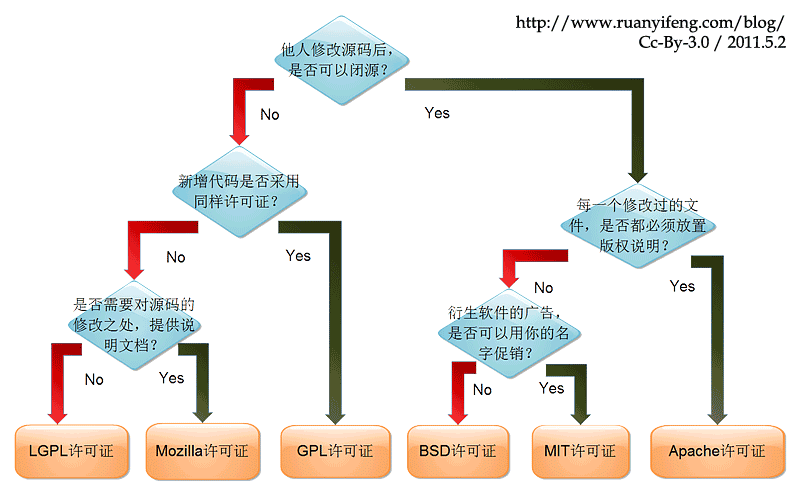
\includegraphics[width=12cm,angle=0]{figures/OpenSource.png}
%height 指定图片的高度
%width 指定图片的宽度
%angle 指定图片旋转的角度
%scale 缩放图形
\caption{Example twig query and documents }     %插入图片的标题,一般放在图片的下方,放在表格的上方
\label{fig_example1}
\end{figure}


\section{公式}
论文中的出现的公式有两种:一种是行内公式,另一种是行间居中公式。
\subsection{行内公式}
书写行内公式时只需要将公式代码放入两个\$符号中间即可,公式与行的间距将自动调整。这也是一个比Word 更方面的一个功能。比如:质能方程$E=mc^2$。
\subsection{行间公式}
书写行间方式可以将公式代码放入两个\$\$符号中间,此时无法对公式进行编号。比如:质能方程$$E=mc^2$$\par
也可以放入$\backslash$ begin\{equation\} 和 $\backslash$ end\{equation\}之间,使用此命令可以为公式进行编号,对公式进行引用等。比如:质能方程 \ref{eq1}
\begin{equation}\label{eq1}
E=mc^2
\end{equation}


%第四章
% !Mode:: "TeX:UTF-8"

\chapter{��������}
\section{\BibTeX ��ʹ��}
\BibTeX ��һ�ָ�ʽ��һ����������Э��LaTeX�IJο����״�����\BibTeX ʹ�����ݿ�ĵķ�ʽ�������ο�����. \BibTeX �ļ��ĺ�׺��Ϊ .bib�� ������һ�����ӣ�
\begin{quote}
@article\{name1,\\
author = \{����, ��������� and ����\},\\
title = \{����\},\\
journal = \{�ڿ���\},\\
volume = \{��20\},\\
number = \{ҳ��\},\\
year = \{���\},\\
abstract = \{ժҪ, �����Ҫ�����õ�ʱ���Լ��ο���, ��һ�в��DZ����\}\\
\}\\

@book\{name2,\\
author ="����",\\
year="���2008",\\
title="����",\\
publisher ="����������"\\
\}
\end{quote}
˵��:��һ��@article ���� \BibTeX ����һ���������͵IJο����ף�����������ʽ, ���� article, book, booklet, conference, inbook, incollection, inproceedings��manual, misc, mastersthesis, phdthesis, proceedings, techreport, unpublished �ȵȡ���������"name1"����������������Ӧ�������Ŀ�����ơ��������Dzο���������ľ�����������
\section{��\LaTeX��ʹ��\BibTeX}
Ϊ����LaTeX��ʹ��BibTeX ���ݿ�, ���������������������:
\begin{enumerate}
\item ���òο����׵����� (bibliography style). ��׼��Ϊ plain:\\
����$\backslash$bibliographystyle\{plain\}\\
�������������� \LaTeX �ĵ��� $\backslash$begin\{document\}���. ���������Ͱ���:\\
unsrt �C �����ϸ� plain ����һ�������˲ο����׵���Ŀ�ı���ǰ������õ�˳�򣬶����ǰ������ߵ���ĸ˳��\\
alpha �C ������ plain ���ͣ����ο����׵���Ŀ�ı�Ż����������ֺͳ�����ݵ�˳��\\
abbrv �C ��д��ʽ��
\item ������� (Make citations). �������ĵ�����ʹ������ʱ, ����\LaTeX ����$\backslash$cite{������������}��"������������" ����ǰ�߶���@article���������.
\item ����LaTeX���ɲο������б����� LaTeX �Ľ���ǰ����$\backslash$bibliography{bibfile}������bibfile ������� BibTeX ���ݿ��ļ� bibfile.bib .
\end{enumerate}

\section{���� \BibTeX}
�������IJ�:
\begin{enumerate}
\item ��LaTeX������� .tex �ļ� , ��������һ�� .aux ���ļ�, ����� \BibTeX ��ʹ����ЩӦ�ã�
\item ��\BibTeX ���� .bib �ļ���
\item �ٴ���\LaTeX ������� .tex �ļ������ʱ�����ĵ����Ѿ������˲ο����ף�����ʱ���õı�ſ��ܲ���ȷ��
\item ����� \LaTeX ������� .tex �ļ������һ��˳���Ļ�, �������ж�������������.
\end{enumerate}

\section{�����IJο����׸�ʽ}
�����Ƽ���ѧ��ʿ���ĵIJο�����Ҫ����Ϲ��ұ�׼��GB/T7714-2005�ĺ�ο�������¼���򡱡���ģ�����Ѱ����˹��ڷ��ϴ�Ҫ���gbt7714-2005.bst�ļ���ֻ��Ҫ���ο�������������Ϊ$\backslash$bibliographystyle\{gbt7714-2005\}���ɡ�



\addcontentsline{toc}{chapter}{参考文献}  %在目录中添加“参考文献”的标记
\bibliographystyle{gbt7714-2005}
\bibliography{ref}

%附录(如不需要请注释掉)
% !Mode:: "TeX:UTF-8"

\chapter*{\centering 附录}

此部分内容并非必须,如需删除请在main.tex中注释掉即可。

%作者简历及在学研究成果
% !Mode:: "TeX:UTF-8"

\chapter*{\centering ���߼�������ѧ�о��ɹ�}

\noindent һ��������ѧǰ���� \par
%��ʿ��ѧǰ�����������Լ������д����ע����дְ��ȡ�
\vspace{2ex}
\begin{tabular}{|c|c|c|}\hline
��ֹ���� & ѧϰ������λ & ��ע \\ \hline
XXXX��XX����XXXX��XX�� & ��XXXX ѧУXXXX רҵ����ѧʿѧλ &  \\ \hline
XXXX��XX����XXXX��XX�� & ��XXXX ѧУXXXX רҵ����˶ʿѧλ &  \\ \hline
XXXX��XX����XXXX��XX�� & ��XXXX ��λ����XXXX ��λ�Ĺ��� &  \\ \hline
\end{tabular} 

\noindent ������ѧ�ڼ���µĿ��й��� \par
%��Ӧע���������ơ��μ����ݡ�ͨ��ʱ�䡢ͨ����ʽ��������λ�ȣ���
\begin{enumerate}
\item ˶ʿ��ʿ��ҵ����\LaTeX ģ��ı�д��\\
��Ϊ��Ҫ�༭�ˣ���2016��3�·ݿ�ʼ��������Ŀ����һֱ�����޸ģ�ϣ��������һ�������ģ�岢�ұ��ٷ��Ͽɡ�
\end{enumerate}
\noindent ������ѧ�ڼ�����Ŀ��н��� \par
%Ӧע���������ơ��ڽ���λ���ڽ�ʱ��ȣ�����д���з��潱����������д����������Ϣ���粻����д�����о����Ƚ�����Ϣ����
\par
\noindent �ġ���ѧ�ڼ䷢�������� \par
%Ӧ���ղο����׵ĸ�ʽ����д��������š����ں������α��������������֮���á������ָ���1���������ѷ���������¼�á���2���Ƿ�SCI/EI/STP/CSSCI ��Դ����3���Ƿ񱻡�SCI/EI/STP/CSSCI ��������4�������š��� 2��3 �����������������ƣ���






%ä�����ģ�����ȥ���п���Ӱ��ä��������Ϣ������������������ʦ����������ѧ�ŵȡ������ڴ˴����о��ɹ����������ߵķ��������б���Ӧ��ȥ�������ߵ����֣�ֻ�������������ǵڼ����ߣ������硰[�ڶ�����]���������ƣ�������

%独创性说明和关于论文使用授权的说明
% !Mode:: "TeX:UTF-8"

\chapter*{\centering 独创性说明}
\doublespacing
本人郑重声明:所呈交的论文是我个人在导师指导下进行的研究工作及取得研究成果。尽我所知,除了文中特别加以标注和致谢的地方外,论文中不包含其他人已经发表或撰写的研究成果,也不包含为获得北京科技大学或其他教育机构的学位或证书所使用过的材料。与我一同工作的同志对本研究所做的任何贡献均已在论文中做了明确的说明并表示了谢意。\par

\vspace{3ex}

\begin{flushright}
签名:\underline{\makebox[3cm]{\qquad}} 日期:\underline{\makebox[3cm]{\qquad}}
\end{flushright}

\vspace{10ex}

\begin{center}
{\zihao{-1} 关于论文使用授权的说明} 
\end{center}
\par

\vspace{5ex}


本人完全了解北京科技大学有关保留、使用学位论文的规定,即:学校有权保留送交论文的复印件,允许论文被查阅和借阅;学校可以公布论文的全部或部分内容,可以采用影印、缩印或其他复制手段保存论文。\par
(保密的论文在解密后应遵循此规定)\par

\vspace{3ex}

\begin{flushright}
签名:\underline{\makebox[3cm]{\qquad}} 导师签名:\underline{\makebox[3cm]{\qquad}}日期:\underline{\makebox[3cm]{\qquad}}
\end{flushright}


%学位论文数据集
% !Mode:: "TeX:UTF-8"

\chapter*{\centering 学位论文数据集}
\begin{table}[htbp]
\centering
\zihao{5} \noindent\makebox[\textwidth]{%
\begin{tabularx}{1.1\textwidth}{|X|X|X|X|X|}
\toprule
关键词* & 密级* & 中国分类号* & UDC & 论文资助 \\ \hline
    &   &   &   &   \\
\midrule
\multicolumn{2}{|l|}{学位授予单位名称* } & 学位授予单位代码* & 学位类别* & 学位级别* \\ \hline
\multicolumn{2}{|l|}{\UniversityCN } & 10008 &  工学 & \degreecn \\
\midrule
\multicolumn{2}{|l|}{论文题名* } & \multicolumn{2}{|l|}{并列题名  } & 论文语种* \\ \hline
\multicolumn{2}{|l|}{\ThesisTitleCN }  & \multicolumn{2}{|l|}{ } & 汉语 \\
\midrule
作者姓名*   & \multicolumn{2}{|l|}{\AuthorCN }    & 学号*   &   \StudentID \\
\midrule
\multicolumn{2}{|l|}{培养单位名称*  } & 培养单位代码*  & 培养单位地址  & 邮编 \\ \hline
\multicolumn{2}{|l|}{\UniversityCN } & 10008 &  北京市海淀区学院路30号 & 100083 \\
\midrule
\multicolumn{2}{|l|}{学科专业*} & 研究方向*   & 学制*  & 学位授予年* \\ \hline
\multicolumn{2}{|l|}{\MajorCN } &  &  4 & 2016 \\
\midrule
论文提交日期* & \multicolumn{4}{|l|}{\date } \\     %日期可以自由填写,并不一定是\date
\midrule
导师姓名*    & \multicolumn{2}{|l|}{\TeacherCN ,\SubTeacherCN }    & 职称*    &   \TeacherJobtitle , \SubTeacherJobtitle \\
\midrule
评阅人    & \multicolumn{2}{|l|}{答辩委员会主席* }    & \multicolumn{2}{|l|}{答辩委员会成员 } \\ \hline
   & \multicolumn{2}{|l|}{}    & \multicolumn{2}{|l|}{ } \\
\midrule
\multicolumn{5}{|l|}{电子版论文提交格式 \quad 文本(\quad)图像(\quad)视频(\quad)音频(\quad)多媒体( \quad )其他( \quad )} \\
\multicolumn{5}{|l|}{推荐格式:application/msword;application/pdf} \\
\midrule
\multicolumn{2}{|l|}{电子版论文出版(发布)者  } & \multicolumn{2}{|l|}{电子版论文出版(发布)地  } & 权限声明\\ \hline
\multicolumn{2}{|l|}{} & \multicolumn{2}{|l|}{} & \\
\midrule
论文总页数* & \multicolumn{4}{|l|}{\pageref{LastPage}-3} \\ \hline
\multicolumn{5}{|l|}{共 33 项,其中带*为必填数据,为 22 项。} \\
\bottomrule
\end{tabularx}}
\end{table}


\end{document}
